\section{User Interface}
\label{sec:inference:user_interface}

The \acrfull{ui} is designed to be simple and modern.
It features two different layouts: a bootsplash screen and an inference screen.
The bootsplash screen shows information about the boot process (e.g. initialization messages, error messages) and the inference screen shows the classification results of the latest throw.
No user input is required, as the application is almost immediately ready again after displaying the results of the latest throw.

% ------------------------------------------------------------------------------------------------------------------------------
\subsection{Bootsplash Screen}
\label{subsec:inference:user_interface:bootsplash_screen}

The bootsplash screen is displayed during the initialization phase of the application.
It consists of the FHNW logo in the top left corner, the title of the project, the names of the project authors and a configurable status message.
The configurable status message is used to display both initialization messages and camera error messages.

A bootsplash screen with an initialization status message is shown in figure \ref{fig:ui_boot}.

\begin{figure}
  \centering
  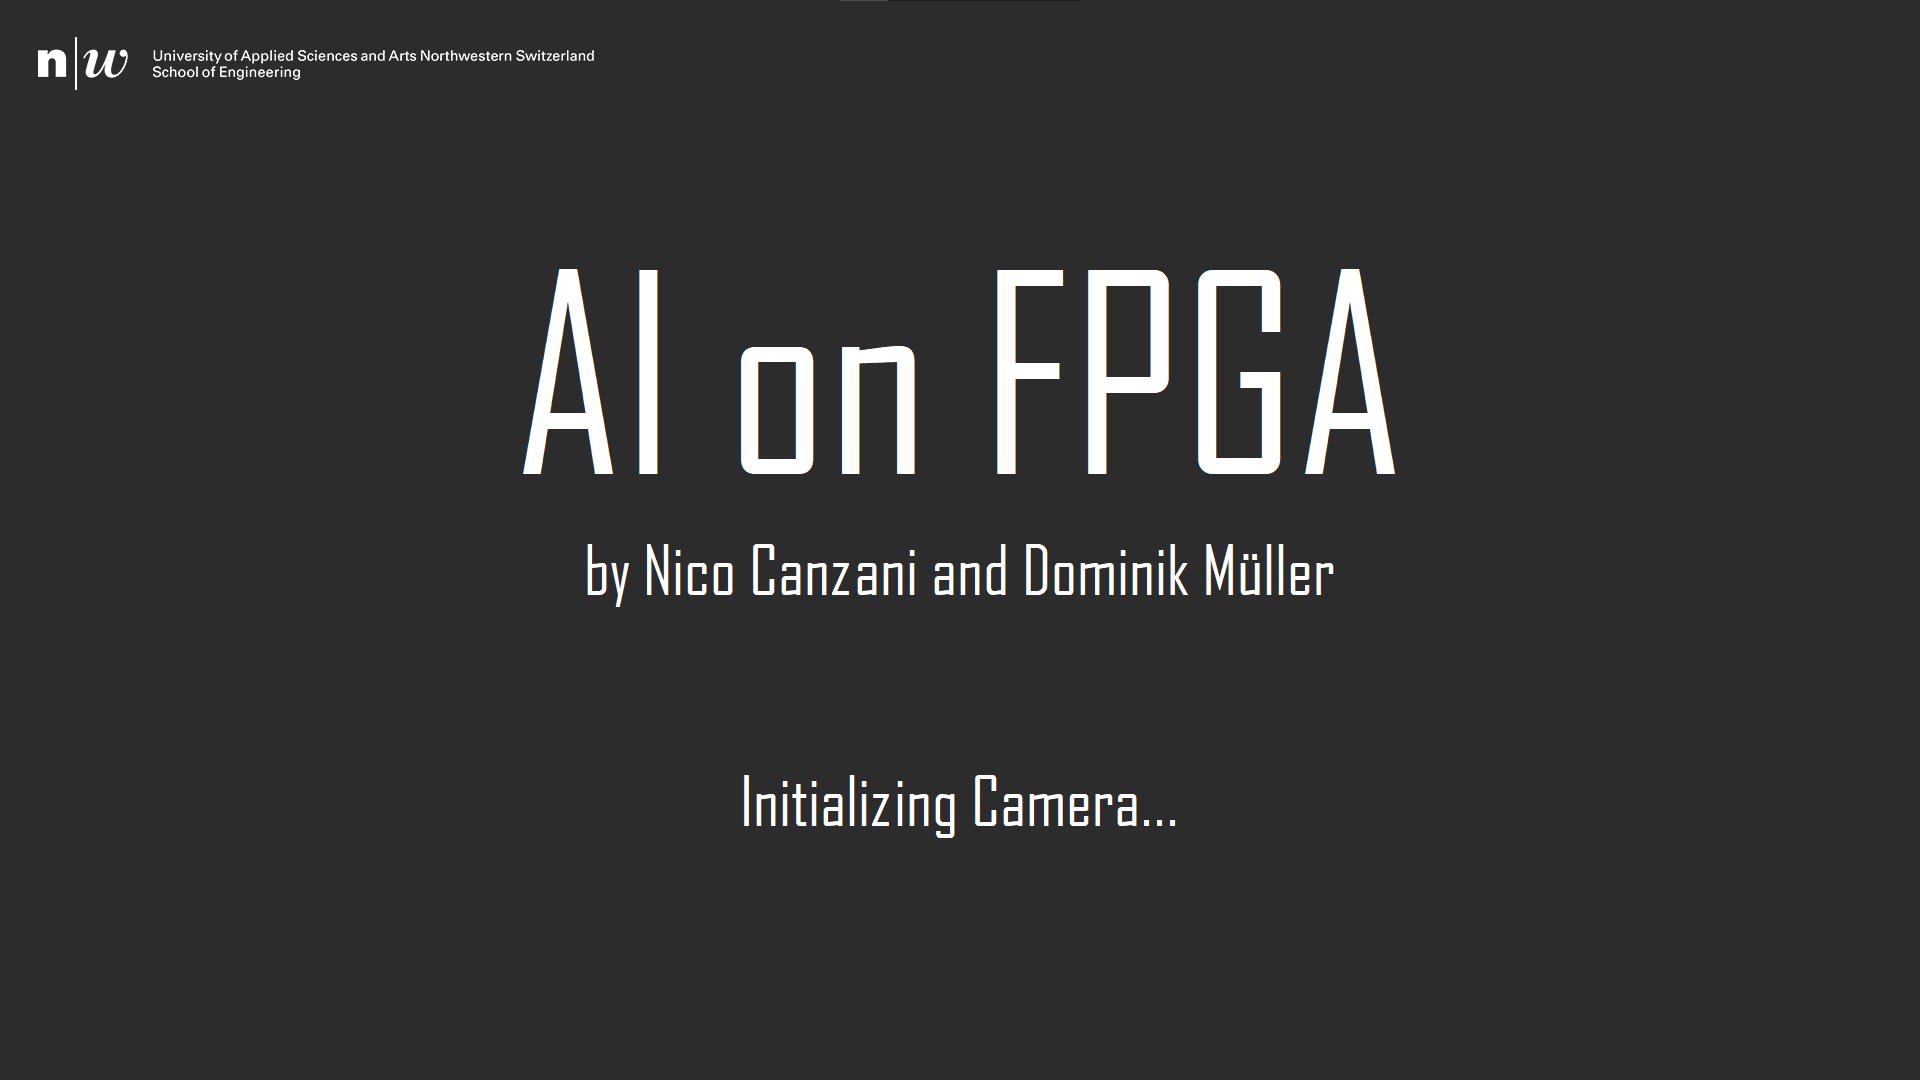
\includegraphics[width=\textwidth]{ui/ui_boot}
  \caption{Bootsplash screen with a camera initialization message}
  \label{fig:ui_boot}
\end{figure}

% ------------------------------------------------------------------------------------------------------------------------------
\subsection{Inference Screen}
\label{subsec:inference:user_interface:inference_screen}

The inference screen is displayed after a detected throw has been evaluated.
It consists of the FHNW logo in the top left corner, an acquired image of the object on the left half of the screen and the classification statistics on the right half of the screen.

The displayed image of the object is the one with the highest weighted prediction percentage of the class selected as the best prediction.
This is most likely a frame from the middle of the throw due to the applied weighting (see section \ref{subsec:inference:app:ui}).

The classification statistics are visualized in a donut chart which shows the best prediction, up to three additional predictions and the sum of the rest of the prediction percentages.
Additional predictions are only shown if their percentages are greater or equal to \SI{1.0}{\percent}.
Furthermore, the sum of the rest of the percentages is only shown if it is not equal to zero after rounding.
All percentages are rounded to one decimal place before being displayed (see section \ref{subsec:inference:app:ui}).

Displaying the throughput of the image classification chain in frames per second is not necessary as it remains more or less constant.
The small differences are due to background tasks of the Linux operating system (see section \ref{sec:verification_and_benchmark:throughput}).

Figure \ref{fig:ui_inference_paper_ball} show an example of the inference screen.
The classification accuracy, however, reaches \SI{100.0}{\percent} in most cases.
Therefore, the inference screen usually looks more like the one shown in figure \ref{fig:ui_inference_bunny}.

\begin{figure}
  \centering
  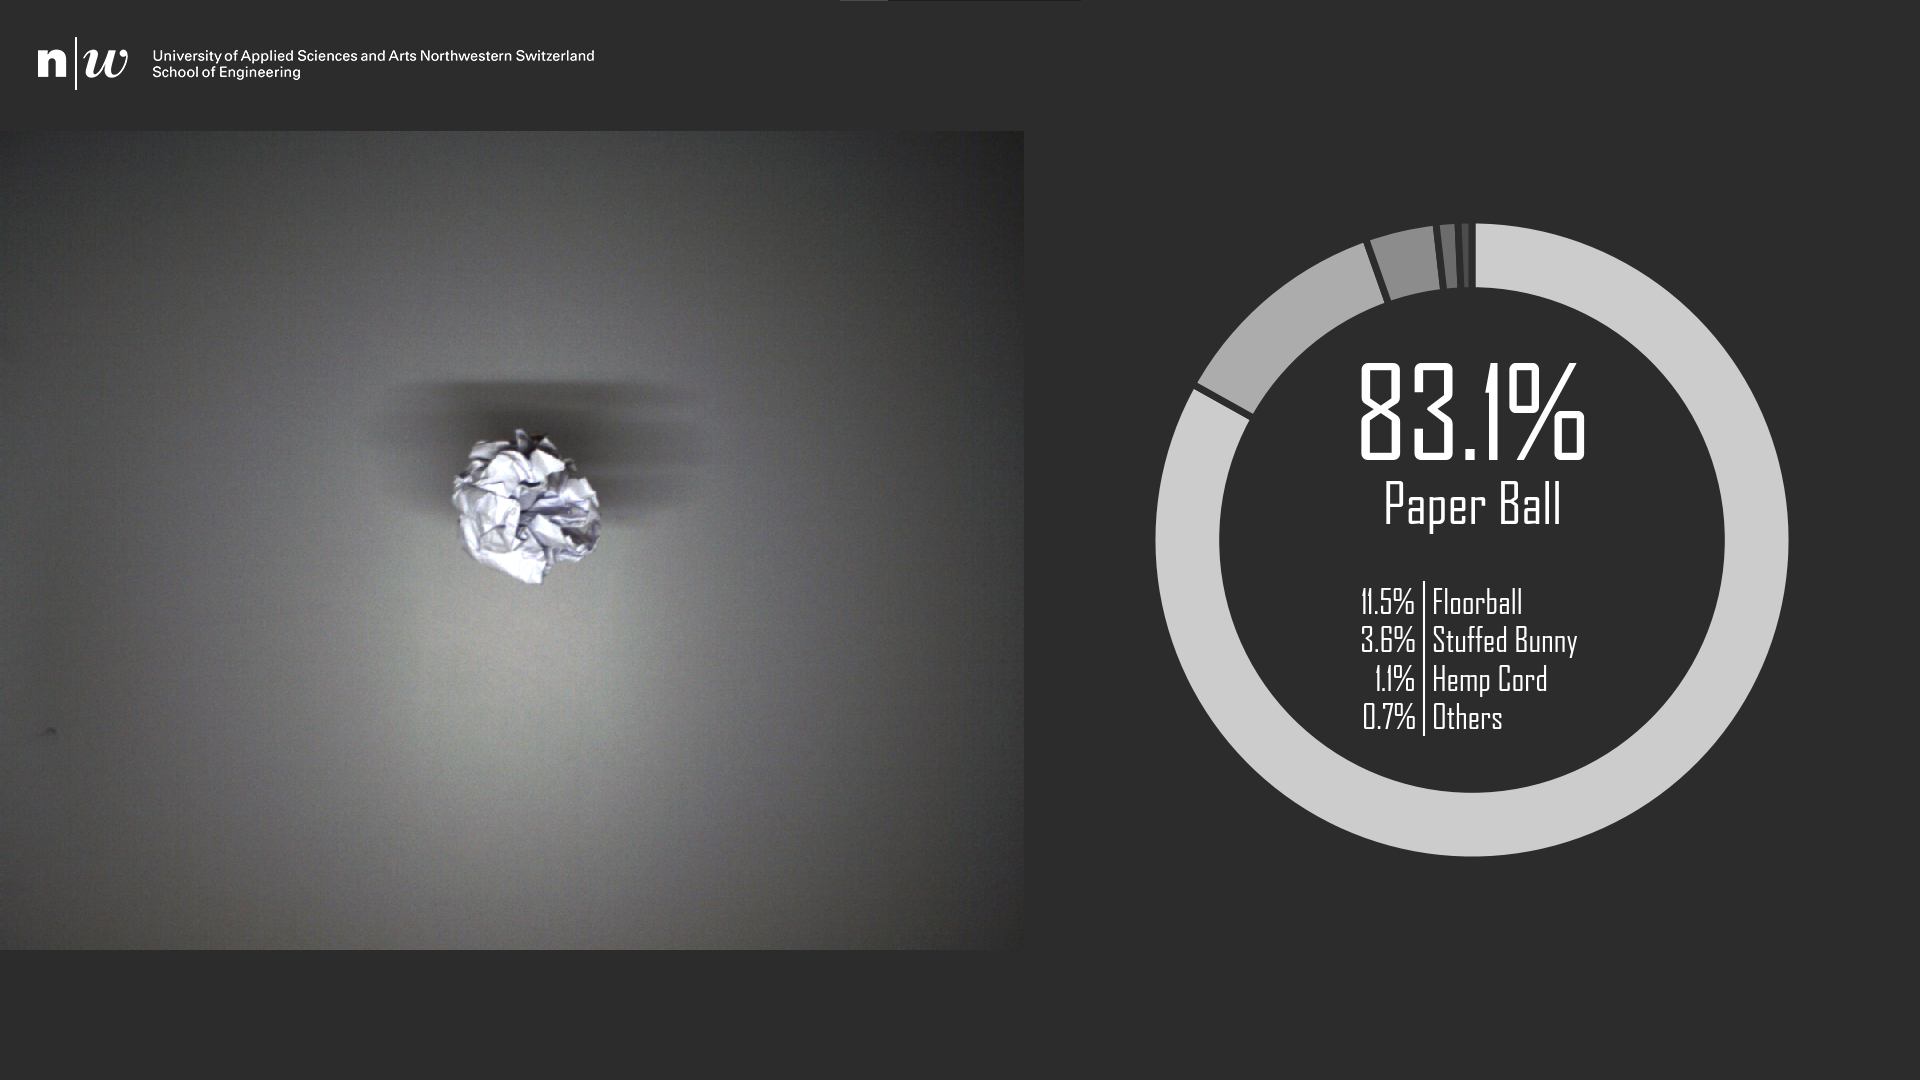
\includegraphics[width=\textwidth]{ui/ui_inference_paper_ball}
  \caption{Example of an inference screen showing the \textit{Paper Ball}}
  \label{fig:ui_inference_paper_ball}
\end{figure}

\begin{figure}
  \centering
  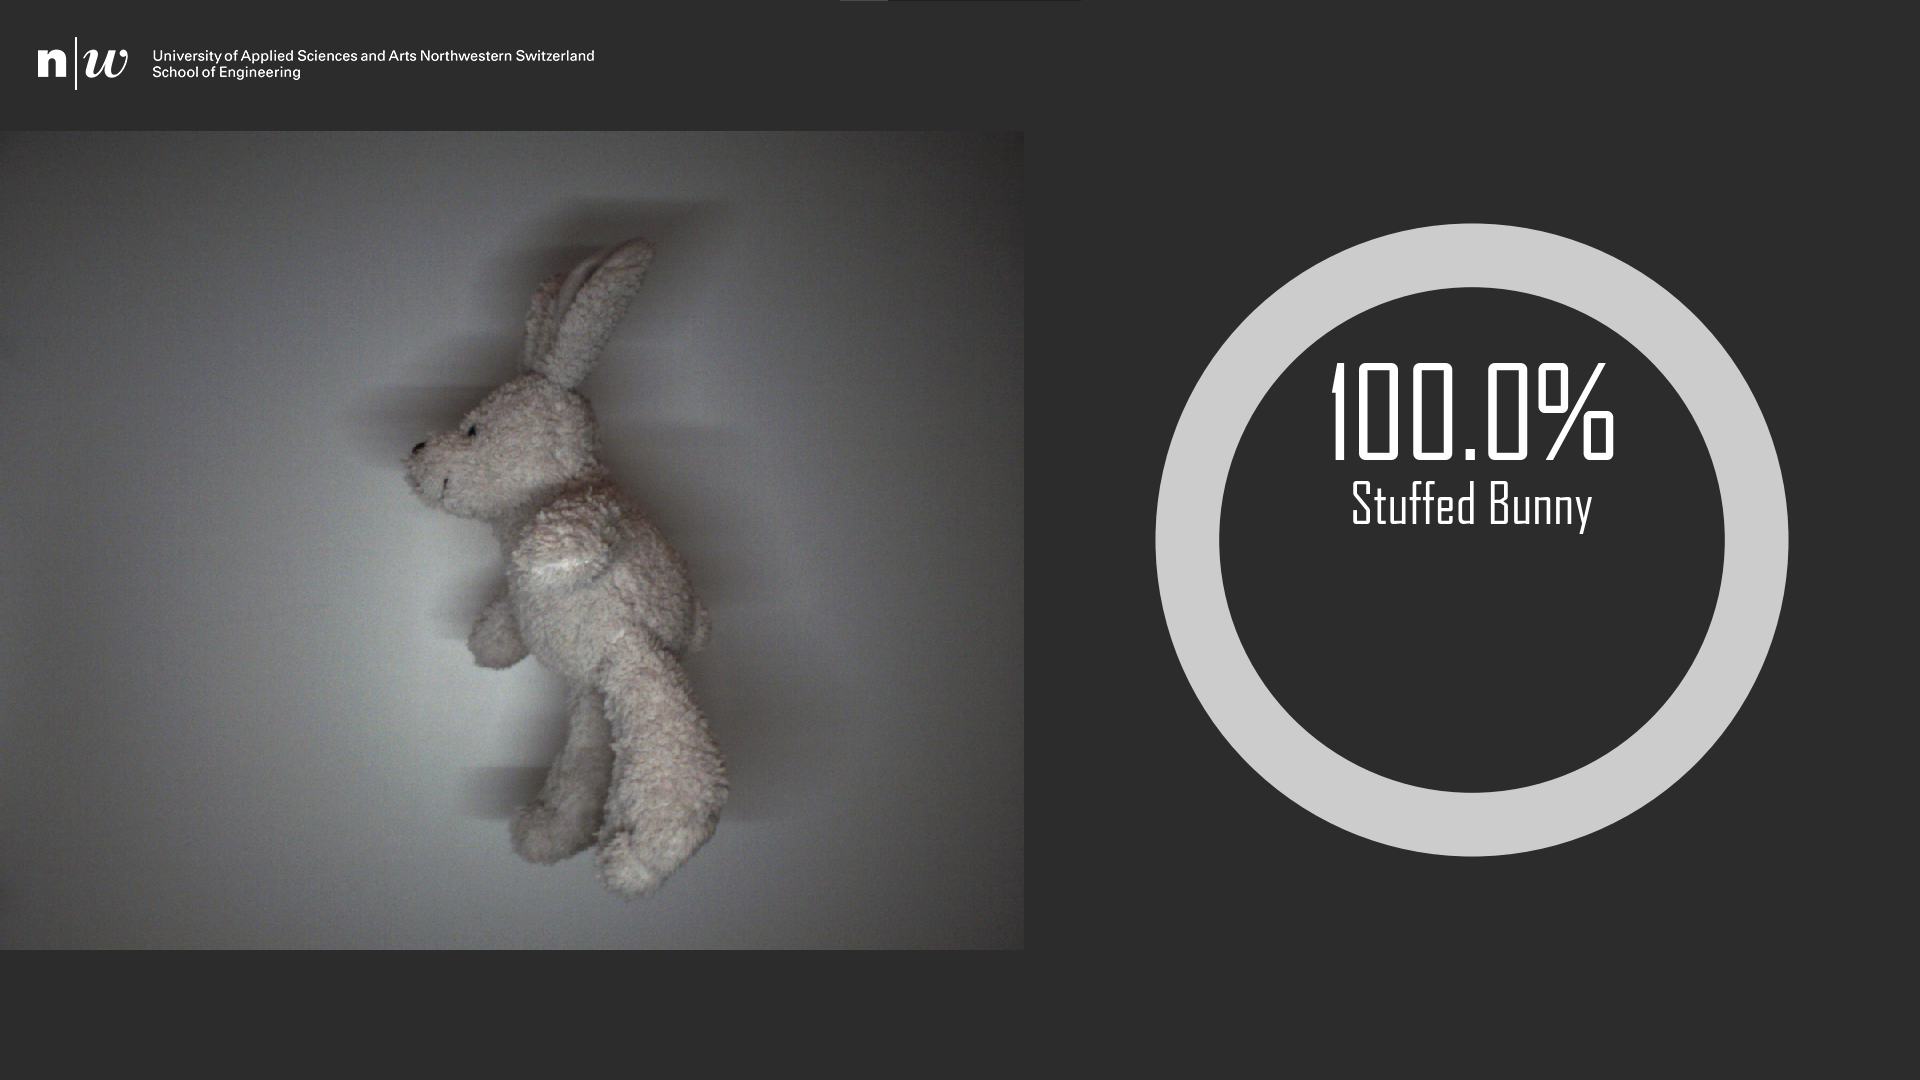
\includegraphics[width=\textwidth]{ui/ui_inference_bunny}
  \caption{Example of an inference screen with a prediction of \SI{100.0}{\percent}}
  \label{fig:ui_inference_bunny}
\end{figure}

% ------------------------------------------------------------------------------------------------------------------------------
\subsection{Implementation}
\label{subsec:inference:user_interface:implementation}

The \acrlong{ui} is implemented as a class in the Python module \texttt{ui.py} and uses the Python packages PySimpleGUI as well as Matplotlib.

PySimpleGUI allows for the creation of simple \acrlongpl{ui} that work across multiple platforms.
Currently, there exist four ports of PySimpleGUI and the Tkinter variant is used by default \cite{inf_pysimplegui}.
Tkinter is the standard Python interface to the Tk cross-platform widget toolkit that provides a library of graphical widgets to build \acrlongpl{ui} \cite{inf_tkinter}.

Matplotlib is a flexible plotting library which provides a MATLAB-like interface with the \texttt{pyplot} module.
Even though it is extremely easy to use, full control over the various properties is not sacrificed as low-level commands are also available \cite{inf_matplotlib}.

% ------------------------------
\paragraph{User Interface Class}
The \texttt{UI} class consists of several non-blocking methods to update the \acrlong{ui} screens.
Calling the PySimpleGUI \texttt{read} method of the \texttt{Window} class is used to update the screens.
However, this call blocks the Python interpreter until a user event occurs (e.g. a button click).
This standard \acrlong{ui} behaviour would render the entire package unusable.
Fortunately, the \texttt{read} method allows to specify a timeout, which essentially turns it into polling mode.
It is therefore called with a short timeout of \SI{100}{ms}, which is necessary to update the screen \cite{inf_pysimplegui_ref}.

The \texttt{boot\_window} and \texttt{inference\_window} methods are used to spawn windows with the appropriate layouts described in section \ref{subsec:inference:user_interface:bootsplash_screen} and \ref{subsec:inference:user_interface:inference_screen}.

The main methods are \texttt{update\_boot\_window} and \texttt{update\_inference\_window}.
When called, they first check whether the screen layout is set to the requested one and switch to it if necessary.
The \acrlong{ui} screen is then updated in a second step and requires the status message in case of the bootsplash screen.
Updating the inference screen requires a list of the predictions, a list of the prediction percentages and the \acrshort{png} encoded image data.

% -----------------------------------
\paragraph{Classification Statistics}
The \texttt{figure} method uses Matplotlib to turn the classification statistics into a donut chart.
Directly generating a donut chart is, however, not possible with Matplotlib.
Therefore, a circle with the same color as the background is placed in the middle of a pie chart.
This simple modification creates the desired donut chart.

To display the figure on the screen, it must be in the \acrshort{png} file format.
For this reason, it is saved to an in-memory \texttt{bytes} buffer to avoid slow file operations.
This is implemented in the \texttt{get\_img\_from\_figure} method.

Animating the ring of the donut chart with Matplotlib would easily be possible by rendering several versions of it overlaid with a circular sector in the background color.
As time passes, the central angle of the circular sector is decreased, starting at the top of the ring and progressing in a clockwise direction around the ring.
This would give the appearance that the ring is being drawn on the display.
Unfortunately, the processor of the embedded system is not powerful enough to render several versions of the donut chart in a reasonable amount of time.

% ----------------
\paragraph{Cursor}
The cursor cannot be disabled globally, but it is possible to hide it when it is hovering over certain elements (e.g. text, images).
For this purpose, the underlying Tkinter widgets are accessed with the \texttt{Widget} class variable and the cursor is set to invisible \cite{inf_pysimplegui_widget}.
The cursor position is centered on the screen after booting.
Therefore, the respective Tkinter widgets located in the center are modified to hide the cursor.
